\documentclass[journal,comsoc]{IEEEtran}
\usepackage[T1]{fontenc}% optional T1 font encoding


% Some very useful LaTeX packages include:
% (uncomment the ones you want to load)


\usepackage{float}


% *** CITATION PACKAGES ***
%
\usepackage{cite}
% cite.sty was written by Donald Arseneau
% V1.6 and later of IEEEtran pre-defines the format of the cite.sty package
% \cite{} output to follow that of the IEEE. Loading the cite package will
% result in citation numbers being automatically sorted and properly
% "compressed/ranged". e.g., [1], [9], [2], [7], [5], [6] without using
% cite.sty will become [1], [2], [5]--[7], [9] using cite.sty. cite.sty's
% \cite will automatically add leading space, if needed. Use cite.sty's
% noadjust option (cite.sty V3.8 and later) if you want to turn this off
% such as if a citation ever needs to be enclosed in parenthesis.
% cite.sty is already installed on most LaTeX systems. Be sure and use
% version 5.0 (2009-03-20) and later if using hyperref.sty.
% The latest version can be obtained at:
% http://www.ctan.org/pkg/cite
% The documentation is contained in the cite.sty file itself.





\usepackage{graphicx}
% *** GRAPHICS RELATED PACKAGES ***
%
\ifCLASSINFOpdf
  % \usepackage[pdftex]{graphicx}
  % declare the path(s) where your graphic files are
  % \graphicspath{{../pdf/}{../jpeg/}}
  % and their extensions so you won't have to specify these with
  % every instance of \includegraphics
  % \DeclareGraphicsExtensions{.pdf,.jpeg,.png}
\else
  % or other class option (dvipsone, dvipdf, if not using dvips). graphicx
  % will default to the driver specified in the system graphics.cfg if no
  % driver is specified.
  % \usepackage[dvips]{graphicx}
  % declare the path(s) where your graphic files are
  % \graphicspath{{../eps/}}
  % and their extensions so you won't have to specify these with
  % every instance of \includegraphics
  % \DeclareGraphicsExtensions{.eps}
\fi
% graphicx was written by David Carlisle and Sebastian Rahtz. It is
% required if you want graphics, photos, etc. graphicx.sty is already
% installed on most LaTeX systems. The latest version and documentation
% can be obtained at: 
% http://www.ctan.org/pkg/graphicx
% Another good source of documentation is "Using Imported Graphics in
% LaTeX2e" by Keith Reckdahl which can be found at:
% http://www.ctan.org/pkg/epslatex
%
% latex, and pdflatex in dvi mode, support graphics in encapsulated
% postscript (.eps) format. pdflatex in pdf mode supports graphics
% in .pdf, .jpeg, .png and .mps (metapost) formats. Users should ensure
% that all non-photo figures use a vector format (.eps, .pdf, .mps) and
% not a bitmapped formats (.jpeg, .png). The IEEE frowns on bitmapped formats
% which can result in "jaggedy"/blurry rendering of lines and letters as
% well as large increases in file sizes.
%
% You can find documentation about the pdfTeX application at:
% http://www.tug.org/applications/pdftex





% *** MATH PACKAGES ***
%
\usepackage{amsmath}
% A popular package from the American Mathematical Society that provides
% many useful and powerful commands for dealing with mathematics.
% Do NOT use the amsbsy package under comsoc mode as that feature is
% already built into the Times Math font (newtxmath, mathtime, etc.).
% 
% Also, note that the amsmath package sets \interdisplaylinepenalty to 10000
% thus preventing page breaks from occurring within multiline equations. Use:
\interdisplaylinepenalty=2500
% after loading amsmath to restore such page breaks as IEEEtran.cls normally
% does. amsmath.sty is already installed on most LaTeX systems. The latest
% version and documentation can be obtained at:
% http://www.ctan.org/pkg/amsmath


% Select a Times math font under comsoc mode or else one will automatically
% be selected for you at the document start. This is required as Communications
% Society journals use a Times, not Computer Modern, math font.
\usepackage[cmintegrals]{newtxmath}
% The freely available newtxmath package was written by Michael Sharpe and
% provides a feature rich Times math font. The cmintegrals option, which is
% the default under IEEEtran, is needed to get the correct style integral
% symbols used in Communications Society journals. Version 1.451, July 28,
% 2015 or later is recommended. Also, do *not* load the newtxtext.sty package
% as doing so would alter the main text font.
% http://www.ctan.org/pkg/newtx
%
% Alternatively, you can use the MathTime commercial fonts if you have them
% installed on your system:
%\usepackage{mtpro2}
%\usepackage{mt11p}
%\usepackage{mathtime}


%\usepackage{bm}
% The bm.sty package was written by David Carlisle and Frank Mittelbach.
% This package provides a \bm{} to produce bold math symbols.
% http://www.ctan.org/pkg/bm





% *** SPECIALIZED LIST PACKAGES ***
%
%\usepackage{algorithmic}
% algorithmic.sty was written by Peter Williams and Rogerio Brito.
% This package provides an algorithmic environment fo describing algorithms.
% You can use the algorithmic environment in-text or within a figure
% environment to provide for a floating algorithm. Do NOT use the algorithm
% floating environment provided by algorithm.sty (by the same authors) or
% algorithm2e.sty (by Christophe Fiorio) as the IEEE does not use dedicated
% algorithm float types and packages that provide these will not provide
% correct IEEE style captions. The latest version and documentation of
% algorithmic.sty can be obtained at:
% http://www.ctan.org/pkg/algorithms
% Also of interest may be the (relatively newer and more customizable)
% algorithmicx.sty package by Szasz Janos:
% http://www.ctan.org/pkg/algorithmicx




% *** ALIGNMENT PACKAGES ***
%
%\usepackage{array}
% Frank Mittelbach's and David Carlisle's array.sty patches and improves
% the standard LaTeX2e array and tabular environments to provide better
% appearance and additional user controls. As the default LaTeX2e table
% generation code is lacking to the point of almost being broken with
% respect to the quality of the end results, all users are strongly
% advised to use an enhanced (at the very least that provided by array.sty)
% set of table tools. array.sty is already installed on most systems. The
% latest version and documentation can be obtained at:
% http://www.ctan.org/pkg/array


% IEEEtran contains the IEEEeqnarray family of commands that can be used to
% generate multiline equations as well as matrices, tables, etc., of high
% quality.




% *** SUBFIGURE PACKAGES ***
%\ifCLASSOPTIONcompsoc
%  \usepackage[caption=false,font=normalsize,labelfont=sf,textfont=sf]{subfig}
%\else
%  \usepackage[caption=false,font=footnotesize]{subfig}
%\fi
% subfig.sty, written by Steven Douglas Cochran, is the modern replacement
% for subfigure.sty, the latter of which is no longer maintained and is
% incompatible with some LaTeX packages including fixltx2e. However,
% subfig.sty requires and automatically loads Axel Sommerfeldt's caption.sty
% which will override IEEEtran.cls' handling of captions and this will result
% in non-IEEE style figure/table captions. To prevent this problem, be sure
% and invoke subfig.sty's "caption=false" package option (available since
% subfig.sty version 1.3, 2005/06/28) as this is will preserve IEEEtran.cls
% handling of captions.
% Note that the Computer Society format requires a larger sans serif font
% than the serif footnote size font used in traditional IEEE formatting
% and thus the need to invoke different subfig.sty package options depending
% on whether compsoc mode has been enabled.
%
% The latest version and documentation of subfig.sty can be obtained at:
% http://www.ctan.org/pkg/subfig




% *** FLOAT PACKAGES ***
%
%\usepackage{fixltx2e}
% fixltx2e, the successor to the earlier fix2col.sty, was written by
% Frank Mittelbach and David Carlisle. This package corrects a few problems
% in the LaTeX2e kernel, the most notable of which is that in current
% LaTeX2e releases, the ordering of single and double column floats is not
% guaranteed to be preserved. Thus, an unpatched LaTeX2e can allow a
% single column figure to be placed prior to an earlier double column
% figure.
% Be aware that LaTeX2e kernels dated 2015 and later have fixltx2e.sty's
% corrections already built into the system in which case a warning will
% be issued if an attempt is made to load fixltx2e.sty as it is no longer
% needed.
% The latest version and documentation can be found at:
% http://www.ctan.org/pkg/fixltx2e


%\usepackage{stfloats}
% stfloats.sty was written by Sigitas Tolusis. This package gives LaTeX2e
% the ability to do double column floats at the bottom of the page as well
% as the top. (e.g., "\begin{figure*}[!b]" is not normally possible in
% LaTeX2e). It also provides a command:
%\fnbelowfloat
% to enable the placement of footnotes below bottom floats (the standard
% LaTeX2e kernel puts them above bottom floats). This is an invasive package
% which rewrites many portions of the LaTeX2e float routines. It may not work
% with other packages that modify the LaTeX2e float routines. The latest
% version and documentation can be obtained at:
% http://www.ctan.org/pkg/stfloats
% Do not use the stfloats baselinefloat ability as the IEEE does not allow
% \baselineskip to stretch. Authors submitting work to the IEEE should note
% that the IEEE rarely uses double column equations and that authors should try
% to avoid such use. Do not be tempted to use the cuted.sty or midfloat.sty
% packages (also by Sigitas Tolusis) as the IEEE does not format its papers in
% such ways.
% Do not attempt to use stfloats with fixltx2e as they are incompatible.
% Instead, use Morten Hogholm'a dblfloatfix which combines the features
% of both fixltx2e and stfloats:
%
% \usepackage{dblfloatfix}
% The latest version can be found at:
% http://www.ctan.org/pkg/dblfloatfix




%\ifCLASSOPTIONcaptionsoff
%  \usepackage[nomarkers]{endfloat}
% \let\MYoriglatexcaption\caption
% \renewcommand{\caption}[2][\relax]{\MYoriglatexcaption[#2]{#2}}
%\fi
% endfloat.sty was written by James Darrell McCauley, Jeff Goldberg and 
% Axel Sommerfeldt. This package may be useful when used in conjunction with 
% IEEEtran.cls'  captionsoff option. Some IEEE journals/societies require that
% submissions have lists of figures/tables at the end of the paper and that
% figures/tables without any captions are placed on a page by themselves at
% the end of the document. If needed, the draftcls IEEEtran class option or
% \CLASSINPUTbaselinestretch interface can be used to increase the line
% spacing as well. Be sure and use the nomarkers option of endfloat to
% prevent endfloat from "marking" where the figures would have been placed
% in the text. The two hack lines of code above are a slight modification of
% that suggested by in the endfloat docs (section 8.4.1) to ensure that
% the full captions always appear in the list of figures/tables - even if
% the user used the short optional argument of \caption[]{}.
% IEEE papers do not typically make use of \caption[]'s optional argument,
% so this should not be an issue. A similar trick can be used to disable
% captions of packages such as subfig.sty that lack options to turn off
% the subcaptions:
% For subfig.sty:
% \let\MYorigsubfloat\subfloat
% \renewcommand{\subfloat}[2][\relax]{\MYorigsubfloat[]{#2}}
% However, the above trick will not work if both optional arguments of
% the \subfloat command are used. Furthermore, there needs to be a
% description of each subfigure *somewhere* and endfloat does not add
% subfigure captions to its list of figures. Thus, the best approach is to
% avoid the use of subfigure captions (many IEEE journals avoid them anyway)
% and instead reference/explain all the subfigures within the main caption.
% The latest version of endfloat.sty and its documentation can obtained at:
% http://www.ctan.org/pkg/endfloat
%
% The IEEEtran \ifCLASSOPTIONcaptionsoff conditional can also be used
% later in the document, say, to conditionally put the References on a 
% page by themselves.




% *** PDF, URL AND HYPERLINK PACKAGES ***
%
%\usepackage{url}
% url.sty was written by Donald Arseneau. It provides better support for
% handling and breaking URLs. url.sty is already installed on most LaTeX
% systems. The latest version and documentation can be obtained at:
% http://www.ctan.org/pkg/url
% Basically, \url{my_url_here}.




% *** Do not adjust lengths that control margins, column widths, etc. ***
% *** Do not use packages that alter fonts (such as pslatex).         ***
% There should be no need to do such things with IEEEtran.cls V1.6 and later.
% (Unless specifically asked to do so by the journal or conference you plan
% to submit to, of course. )


% correct bad hyphenation here
\hyphenation{op-tical net-works semi-conduc-tor}

\usepackage{array}
\usepackage{multirow}

\newcommand\MyBox[2]{
  \fbox{\lower0.75cm
    \vbox to 1.7cm{\vfil
      \hbox to 1.7cm{\hfil\parbox{1.4cm}{#1\\#2}\hfil}
      \vfil}%
  }%
}



\begin{document}
%
% paper title
% Titles are generally capitalized except for words such as a, an, and, as,
% at, but, by, for, in, nor, of, on, or, the, to and up, which are usually
% not capitalized unless they are the first or last word of the title.
% Linebreaks \\ can be used within to get better formatting as desired.
% Do not put math or special symbols in the title.
\title{Feature Selection\\ Fitness Landscape Analysis}
%
%
% author names and IEEE memberships
% note positions of commas and nonbreaking spaces ( ~ ) LaTeX will not break
% a structure at a ~ so this keeps an author's name from being broken across
% two lines.
% use \thanks{} to gain access to the first footnote area
% a separate \thanks must be used for each paragraph as LaTeX2e's \thanks
% was not built to handle multiple paragraphs
%

\author{Werner~Mostert}% <-this % stops a space

% note the % following the last \IEEEmembership and also \thanks - 
% these prevent an unwanted space from occurring between the last author name
% and the end of the author line. i.e., if you had this:
% 
% \author{....lastname \thanks{...} \thanks{...} }
%                     ^------------^------------^----Do not want these spaces!
%
% a space would be appended to the last name and could cause every name on that
% line to be shifted left slightly. This is one of those "LaTeX things". For
% instance, "\textbf{A} \textbf{B}" will typeset as "A B" not "AB". To get
% "AB" then you have to do: "\textbf{A}\textbf{B}"
% \thanks is no different in this regard, so shield the last } of each \thanks
% that ends a line with a % and do not let a space in before the next \thanks.
% Spaces after \IEEEmembership other than the last one are OK (and needed) as
% you are supposed to have spaces between the names. For what it is worth,
% this is a minor point as most people would not even notice if the said evil
% space somehow managed to creep in.



% The paper headers
\markboth{COS 700 Copy}%
{Shell \MakeLowercase{\textit{et al.}}: Bare Demo of IEEEtran.cls for IEEE Communications Society Journals}
% The only time the second header will appear is for the odd numbered pages
% after the title page when using the twoside option.
% 
% *** Note that you probably will NOT want to include the author's ***
% *** name in the headers of peer review papers.                   ***
% You can use \ifCLASSOPTIONpeerreview for conditional compilation here if
% you desire.


% If you want to put a publisher's ID mark on the page you can do it like
% this:
%\IEEEpubid{0000--0000/00\$00.00~\copyright~2015 IEEE}
% Remember, if you use this you must call \IEEEpubidadjcol in the second
% column for its text to clear the IEEEpubid mark.

% use for special paper notices
%\IEEEspecialpapernotice{(Invited Paper)}

% make the title area
\maketitle

% As a general rule, do not put math, special symbols or citations
% in the abstract or keywords.
\begin{abstract}
Feature selection is a complex problem which has been addressed in many different ways. Feature selection algorithms extract a subset of features from an overarching feature set which can greatly improve algorithm performance and accomplish dimensionality reduction. Feature selection algorithms that have been developed are often computationally expensive; provide
an insignificant increase in predictor performance and can lead to overfitting. The paper
investigates the combinatorial problem of selecting feature sets using a given classifier. By analyzing the fitness landscape of the feature selection problem space,
it is envisaged to better understand the problem. Landscape characteristics that have an influence on the search algorithms are investigated.
\end{abstract}

% Note that keywords are not normally used for peerreview papers.
\begin{IEEEkeywords}
Feature Selection, Fitness Landscape, Landscape Analysis
\end{IEEEkeywords}

% For peer review papers, you can put extra information on the cover
% page as needed:
% \ifCLASSOPTIONpeerreview
% \begin{center} \bfseries EDICS Category: 3-BBND \end{center}
% \fi
%
% For peerreview papers, this IEEEtran command inserts a page break and
% creates the second title. It will be ignored for other modes.
\IEEEpeerreviewmaketitle

\section{Introduction}

It is a known fact that humans seemingly effortlessly find patterns in their daily lives. This allows for the perception and detection of arbitrary objects such as other humans and visual keys in the environment. Within the field of machine learning it often attempted to accomplish these goals, since it is of such great value in fields such as computer vision \cite{wernick2010machine}.

Various different classification techniques to date have been developed \cite{nguyen2008survey}, otherwise referred to as classifiers, in order to recognize patterns in data. Classifiers generally work on a similar premise: some conclusion is made with respect to a set of parameters in data. These parameters in the observed data can also be called features. Chandrashekar and Sahin define a feature as "an individual measurable property of the process being observed" \cite{chandrashekar2014survey}. Intuitively speaking, when a human is given the task of recognizing a friend or family member, how can the individual be identified? The human may perhaps take into account physical features such as the person's facial features; voice or even smell. Given the fact that a classifier needs features to perform classification, it becomes a complex problem to decide on which features are the most information rich to provide for a performant classification. Heuristics have been used to great success for classification in combinatorial problems, with little explanation as to why they perform well or not \cite{belaidouni1999landscapes}. The features that are used to perform classification could greatly influence the performance of heuristic techniques.

In order to further the development of a generalized theoretical framework for feature selection and to better understand the feature selection problem this paper analyzes the fitness landscape of the feature selection space with respect to a simple and non-stochastic classifier. Since feature selection is a binary problem, the landscape that is analyzed is discrete. A variety of data sets are considered with varying number of features, types of features and data set sizes.

Section II gives an overview of the feature selection problem and fitness landscape analysis. Landscape characteristics that are considered in this paper are discussed in Section III. Section IV describes the details of conducting the fitness landscape analysis for the feature selection problem and analyzing landscape characteristics. Finally, the experimental results are given.

\section{Feature Selection}
The feature selection problem is that of selecting a subset of all available features. Feature selection is beneficial in order to better understand and visualize data as well as improving classification performance by effectively reducing the dimensionality of the problem \cite{guyon2003introduction}. Modern problems such as image classification suffers from extremely high dimensionality, thus affecting classifier performance. There exist many approaches of feature selection, of which many have proven to be problem dependent and have had varying measures of success \cite{chandrashekar2014survey}.

Since choosing a subset of features from the complete feature set $F$ is a combinatorial problem, the subset $F_s \subseteq F$ can be represented as a binary string $S_i$. An 'on' bit in the string represents the inclusion of the feature, whereas conversely, an 'off' represents its exclusion. In this format it is possible to model a full permutation of all possible inclusions and exclusions of subsets, of the complete feature set $F$. In order to analyze a fitness landscape, the precondition is that it is computationally possible to calculate a fitness value at a given point in the landscape, $f(S_i)$, where $f$ is the fitness function. A unique bit string is referred to as a "problem instance" within the context of this paper.

The issue of feature irrelevance comes to light since two features that are considered within mutual exclusion, could be useless, but the union of these features could be of massive importance \cite{guyon2003introduction}. A primitive approach to solving this problem would be to do an exhaustive search of the combination of features, which results in optimal performance. Given a small number of features this is conceptually possible, however,  as stated by Amaldi  \textit{et al}. \cite{amaldi1998approximability} the full permutation of feature sets for a highly dimensional problem is a non-polynomial (NP)-hard problem.
There are various feature selection algorithms which have been developed to date, and there is still current research on the topic \cite{kira1992feature, jain1997feature, kohavi1997wrappers, yu2003feature, yeh2016feature, ge2016mctwo}. These generally fall into three categories namely filter methods, wrapper methods and embedded methods \cite{chandrashekar2014survey}. There is evidently no shortage of algorithms for conducting feature selection. The algorithms are diverse in how the problem is approached, however, there seems to be no theoretical framework in place to guide researchers in making decisions on which algorithms to use \cite{guyon2003introduction}. As stated by Guyon and Elliseeff, feature selection methods may be used to improve classifier performance \cite{guyon2003introduction}. They did however find that for problems of high dimensionality the performance increase is not always significant. Since the feature selection problem is of a complex nature, it is useful to do landscape analysis in order to be able to obtain more detailed understanding of the problem.




\section{Fitness Landscape Characteristics}

An underlying fitness landscape can be a valuable tool for analysis of heuristic search algorithms \cite{pitzer2012comprehensive} since some fitness landscapes possess structural attributes that can lead search algorithms to good or bad solutions \cite{malan2013survey}. There are various characteristics of a fitness landscape that can be investigated and also many different techniques that may be applied in order to analyze these characteristics \cite{malan2013survey}. Fitness landscape characteristics such as fitness distributions, epistasis, neutrality etc. can prove vital in understanding why certain algorithms perform well on sets of problems and why others do not.
A large number of landscape characteristics may be extracted from a landscape. The characteristics that are investigated are indicative of the shape of the discrete landscape.

\subsection{Fitness Distribution}

The fitness distribution characteristic can be calculated by the fitness function alone - dependent on the grouping strategy used. A simple grouping strategy that can be used is to bin the fitness function values into sub-ranges. This is only possible if the upper and lower bounds of the fitness function is known. In the case where the Kappa-statistic is used, a $B$ number of bins can be used to divide the range $[-1,1]$ into bins of equal size. The bins are initialized to a zero count and for each fitness value the corresponding bin's count is incremented during the walk in the landscape. This results in a histogram of number of fitness value instances for a range of fitness values. By constructing the fitness distribution histogram one may profile the problem to answer the question of how many configurations of the combinatorial problem result in a specific range of fitness values. The fitness distribution as calculated here has some similarities with the density of states technique \cite{asselmeyer1996smoothing}.

\subsection{Hamming Distance in a Level}

The hamming distance in a level as proposed by Belaidouni and Hao \cite{belaidouni1999landscapes} is a measurement of the similarity ,or the lack thereof, of problem instances within a range of fitness values. The authors describe a concept called an iso-cost level which is essentially a set of problem instances that correlate to the same fitness value. The distance $D$ in a set $A$  is defined as \cite{belaidouni1999landscapes}, 
$$
	D(A) = \frac{1}{|A^2|} \sum_{(S_i,S_j') \in L^2} d(S_i, S_j')
$$
where $L$ is the iso-cost level and $S_n$ is the $n$-th problem instance within the level. By using the iso-cost levels one could visualize this technique as calculating the disparity in the other relevant dimensions with respect to a thin slice of range in the fitness dimension. This could be viewed as a measure to indicate the width of the landscape \cite{belaidouni1999landscapes}. In the case of the discrete fitness landscape, this essentially gives a measure of if the solutions within the level are clustered around a specific point or are rather more distributed within the search space.

HDIL as originally proposed defines a fitness level per unique cost value. A slight adaptation is made in this paper where instead of considering problem instances of a specific cost (fitness value), a grouping strategy is used for problem instances in the range of the bin sizes as used for the fitness distribution calculation.

\section{Implementation}


\begin{table*}[t]
\centering
\caption{Data Sets}
\label{table1}
\begin{tabular}{|l|l|l|l|l|l|}
\hline
\textbf{Data Set ID \& Name} & \textbf{Nominal Features} & \textbf{Numerical Features} & \textbf{Number of Classes} & \textbf{Number of Data Elements} & \textbf{Number of Features} \\ \hline
Audiology & Yes & No & 24 & 226 & 70 \\ \hline
Balance Scale & Yes & Yes & 3 & 625 & 5 \\ \hline
Breast W & No & Yes & 2 & 699 & 10 \\ \hline
Anneal.ORIG & Yes & Yes & 6 & 898 & 39 \\ \hline
Letter & No & Yes & 26 & 20000 & 16 \\ \hline
\end{tabular}
\end{table*}

\subsection{Fitness Function}
A measure of classification accuracy is used as the fitness value at a problem instance, $S_i$. The choice of fitness function is of paramount importance when conducting fitness landscape analysis since there exists a variant of the landscape for disparate fitness functions and for variations in calculating the fitness based on different notions of neighborhood for the same fitness function \cite{malan2013survey}.

 Fitness functions, i.e. classifiers, that are stochastic in nature such as artificial neural networks using stochastic gradient descent or random decision forests could very likely provide for usable classification accuracy measurements but would introduce noise into the fitness landscape. This is due to the fact that since a stochastic classifier is generally executed multiple times and the resultant mean performance measurement is used. In such a case by reproducing the fitness landscape the difference between resultant error curves within the hyper-dimensional problem space would become fuzzy due to stochasticity. It is desirable to be able to reliably reproduce the same landscape for a static data set since this allows for landscape characteristics that are independent of change in time, or some other external variable that may affect the fitness calculation. Therefore the classic $k$-nearest-neighbor \cite{cunningham2007k}, a simple non-stochastic classifier is used.

In order to obtain a fitness value,, Cohen's Kappa-statistic, a non-biased measure of classification accuracy, is used. Cohen's Kappa is defined as \cite{ben2008comparison}:

\begin{equation}
	K = \frac{P_0 - P_c}{1 - P_c}
\end{equation}

where $P_c$ is the agreement probability as a result of randomness and $P_0$ is the total agreement probability. The concept of agreement probability is quite simple. Given a confusion matrix as in figure \ref{fig:confuse}, the Kappa statistic would be calculated as follows:

$$
P_c = (\frac{86}{100})(\frac{84}{100}) + (\frac{14}{100})(\frac{16}{100}) = 0.0162
$$
$$
P_0 = \frac{75}{100} + \frac{5}{100} = 0.8
$$
\begin{equation}
K = \frac{0.8 - 0.0162}{1 - 0.0162} = 0.7967
\end{equation}
\hfill\\

The rate of agreement in this case is therefore 0.7967. The Kappa statistic ranges from total disagreement at -1 through completely random classification at 0, to 1 which indicates total agreement. The Kappa statistic allows for the level of agreement for each class label to be measured. This is important since for a raw count of correct classification instances, the results may be statistically biased due to an overwhelming presence or absence of a specific class in an observed data set. The Kappa statistic removes the stochastic element in correct classification count \cite{ben2008comparison} and is also a normalized classification measure in the range [-1,1]. 

\begin{figure}[t!]
\centering
\begin{tabular}{ r|c|c|l }
\multicolumn{1}{r}{}
 &  \multicolumn{1}{c}{A}
 & \multicolumn{1}{c}{B}
& \multicolumn{1}{l}{Total} \\
\cline{2-3}
A & 75 & 11 & 86 \\
\cline{2-3}
B & 9 & 5 & 14 \\
\cline{2-3}
\multicolumn{1}{r}{Total}
 &  \multicolumn{1}{c}{84}
 & \multicolumn{1}{c}{16}
& \multicolumn{1}{l}{100}

\end{tabular}
\hfill\\\hfill\\
\caption{Confusion Matrix 1 for 100 samples}
\label{fig:confuse}
\end{figure}

\subsection{Frameworks and Data Sets}

The UC Irvine Machine Learning Repository, which contains a wide variety of data sets that can be used for various machine learning objectives, was used as a source of data sets \cite{UCI}. A total of 5 data sets were used, which contain nominal and numerical data elements or features. No specific preprocessing of the data sets took place. Table \ref{table1} describes the data sets used.

As an implementation framework the Weka Machine Learning software development kit by the University of Waikato was used \cite{weka}. 

\subsection{Random Walk}

One of the core practices of landscape analysis is the concept of sampling the problem space in order to gain sufficient information about the problem space. There are various possible methods to accomplish this task. One such method is uniform sampling. Within the context of discrete landscapes this entails choosing a random bit string which maps to a configuration within the hypercube of all possible configurations, i.e. problem instances. Naively one may convert the bit string of length $N$ to a real value with the formula $x = 2^N-1$ and sample a value from a uniform distribution constrained by 0 and $x$. However, for a large value of $N$ (as is the case for hyper-dimensional problems) this number becomes exponentially large and difficult to deal with. Another possible solution is to decide for each value within the bit string its on or off value based on if its above or below the median of any constrained uniform distribution, such as 0.5 between in the range $[0,1]$

 A uniform sample, though presents an issue. Problems that are of vastly high dimensionality have an excessively large search space and a simple sample with an insufficient number of points sampled with respect to the size of the search space may heed misleading results. Another issue with this approach is the fact that characteristics that are reliant on the concept of neighborhood will be suppressed.

To address the neighborhood issue above, an initial random point is sampled after which the problem space is navigated by flipping a random number $\delta$ of bits in the bit string $S_i$, where $\delta$ is proportional to the dimensionality $I$ of the problem. This would allow the concept of neighborhood to be retained and the search space to not be underutilized. The value of $\delta$ was calculated as $\delta = k_sI$ where $k_s$ is a scaling constant, in this case set as 0.1. 

Taking the above into account, the concept of neighborhood for the random walk can thus be defined as,
$$
	N_i = \{ x | x \in F \, \text{and} \, d_H(x) = \delta \}
$$
where $d_H$ is the hamming distance. 

Another important parameter to the random walk is the number of steps, i.e. the length of the walk. It would not be fair to do walks of the same length, in a discrete landscape, for a problems that differ in the degree of dimensionality. If the same number of steps were taken the larger landscape would be much further explored than the smaller landscape. Therefore, the number of steps to take $w$ was calculated as,
$$
 w = k_w I
$$
where $k_w$ scales the walking distance. This ensured that the same ratio of the landscapes were covered by the walk. In this case $k_w$ was set to 300.

\section{Research Results}

The fitness distributions for each data set, which is the fitness frequency for different fitness levels, are shown in Table \ref{results-raw}. The fitness levels are  decided to be at intervals of 0.2 from 0 to 1. The Kappa statistic, which is used to calculate fitness, does not dictate how it should be interpreted and thus the literature seems to have developed different interpretations. One such interpretation is \cite{altman1990practical}:

\begin{itemize}
\item
Poor - $f(x) < 0.20$
\item
Fair - $0.20 < f(x) \leq 0.40$
\item
Moderate - $0.40 < f(x) \leq 0.60$
\item Good - $0.60 < f(x) \leq 0.80$
\item Very good  -$ 0.80 < f(x) \leq 1.00$
\end{itemize}

Cohen's Kappa statistic is calculated to be a scalar value in the range $[-1,1]$, however for all data sets tested there was no case where the kappa statistic calculated was within the range $[-1,0)$. It is actually quite rare for the calculated Kappa statistic to be less than 0 in practice for classification. This would mean that the observed level of agreement is less than expected level of agreement by chance. The fitness distribution (FD) is normalized to the 0 to 1 range in Table \ref{results-raw} for visual convenience. 

\begin{table}[H]
\centering
\caption{Results}
\label{results-raw}
\begin{tabular}{lll}
\textbf{Data Set 1} & HDIL & Normalized FD \\ \hline
\multicolumn{1}{|l|}{$f(x) <  0.2$} & \multicolumn{1}{l|}{37.2943} & \multicolumn{1}{l|}{0.0765} \\ \hline
\multicolumn{1}{|l|}{0.2 $ < f(x) \leq $ 0.4} & \multicolumn{1}{l|}{35.8924} & \multicolumn{1}{l|}{0.4012} \\ \hline
\multicolumn{1}{|l|}{0.4 $ < f(x) \leq $ 0.6} & \multicolumn{1}{l|}{35.8436} & \multicolumn{1}{l|}{0.4340} \\ \hline
\multicolumn{1}{|l|}{0.6 $ < f(x) \leq $ 0.8} & \multicolumn{1}{l|}{37.0920} & \multicolumn{1}{l|}{0.0882} \\ \hline
\multicolumn{1}{|l|}{0.8 $ < f(x) \leq $ 1.0} & \multicolumn{1}{l|}{0.0000} & \multicolumn{1}{l|}{0.0000} \\ \hline
\textbf{\begin{tabular}[c]{@{}l@{}}Data Set 2\end{tabular}} &  &  \\ \hline
\multicolumn{1}{|l|}{$f(x) < 0.2$} & \multicolumn{1}{l|}{3.8712} & \multicolumn{1}{l|}{0.2313} \\ \hline
\multicolumn{1}{|l|}{0.2 $ < f(x) \leq $ 0.4} & \multicolumn{1}{l|}{3.0076} & \multicolumn{1}{l|}{0.4967} \\ \hline
\multicolumn{1}{|l|}{0.4 $ < f(x) \leq $ 0.6} & \multicolumn{1}{l|}{3.6805} & \multicolumn{1}{l|}{0.2093} \\ \hline
\multicolumn{1}{|l|}{0.6 $ < f(x) \leq $ 0.8} & \multicolumn{1}{l|}{5.0000} & \multicolumn{1}{l|}{0.0627} \\ \hline
\multicolumn{1}{|l|}{0.8 $ < f(x) \leq $ 1.0} & \multicolumn{1}{l|}{0.0000} & \multicolumn{1}{l|}{0.0000} \\ \hline
\textbf{Data Set 3} &  &  \\ \hline
\multicolumn{1}{|l|}{$f(x) < 0.2$} & \multicolumn{1}{l|}{10.0000} & \multicolumn{1}{l|}{0.0030} \\ \hline
\multicolumn{1}{|l|}{0.2 $ < f(x) \leq $ 0.4} & \multicolumn{1}{l|}{0.0000} & \multicolumn{1}{l|}{0.0000} \\ \hline
\multicolumn{1}{|l|}{0.4 $ < f(x) \leq $ 0.6} & \multicolumn{1}{l|}{9.0278} & \multicolumn{1}{l|}{0.0040} \\ \hline
\multicolumn{1}{|l|}{0.6 $ < f(x) \leq $ 0.8} & \multicolumn{1}{l|}{7.6767} & \multicolumn{1}{l|}{0.0183} \\ \hline
\multicolumn{1}{|l|}{0.8 $ < f(x) \leq $ 1.0} & \multicolumn{1}{l|}{5.5266} & \multicolumn{1}{l|}{0.9747} \\ \hline
\textbf{Data Set 4} &  &  \\ \hline
\multicolumn{1}{|l|}{$f(x) < 0.2$} & \multicolumn{1}{l|}{26.9497} & \multicolumn{1}{l|}{0.0022} \\ \hline
\multicolumn{1}{|l|}{0.2 $ < f(x) \leq $ 0.4} & \multicolumn{1}{l|}{22.5481} & \multicolumn{1}{l|}{0.0277} \\ \hline
\multicolumn{1}{|l|}{0.4 $ < f(x) \leq $ 0.6} & \multicolumn{1}{l|}{20.5674} & \multicolumn{1}{l|}{0.2217} \\ \hline
\multicolumn{1}{|l|}{0.6 $ < f(x) \leq $ 0.8} & \multicolumn{1}{l|}{20.0692} & \multicolumn{1}{l|}{0.5892} \\ \hline
\multicolumn{1}{|l|}{0.8 $ < f(x) \leq $ 1.0} & \multicolumn{1}{l|}{21.2160} & \multicolumn{1}{l|}{0.1591} \\ \hline
\textbf{Data Set 5} &  &  \\ \hline
\multicolumn{1}{|l|}{$f(x) < 0.2$} & \multicolumn{1}{l|}{14.4400} & \multicolumn{1}{l|}{0.0010} \\ \hline
\multicolumn{1}{|l|}{0.2 $ < f(x) \leq $ 0.4} & \multicolumn{1}{l|}{11.5693} & \multicolumn{1}{l|}{0.0163} \\ \hline
\multicolumn{1}{|l|}{0.4 $ < f(x) \leq $ 0.6} & \multicolumn{1}{l|}{10.1475} & \multicolumn{1}{l|}{0.1039} \\ \hline
\multicolumn{1}{|l|}{0.6 $ < f(x) \leq $ 0.8} & \multicolumn{1}{l|}{9.1494} & \multicolumn{1}{l|}{0.4192} \\ \hline
\multicolumn{1}{|l|}{0.8 $ < f(x) \leq $ 1.0} & \multicolumn{1}{l|}{9.4104} & \multicolumn{1}{l|}{0.4596} \\ \hline
\end{tabular}
\end{table}

For easy interpretation,Figure 2 shows a graph of the normalized fitness distributions for the various data sets. At this point it may be noted that the fitness distributions differ quite significantly.

Most of the data sets have a low proportion of solutions in the high fitness range (above 0.8 accuracy). Data sets 3 and 5 are exceptions. This indicates that these datasets have a large number of feature selection solutions that give reasonable accuracy levels, and will probably be easier to search for a good solution.

\begin{figure}[H]
\label{fitness-dist}
\caption{Fitness Distribution}
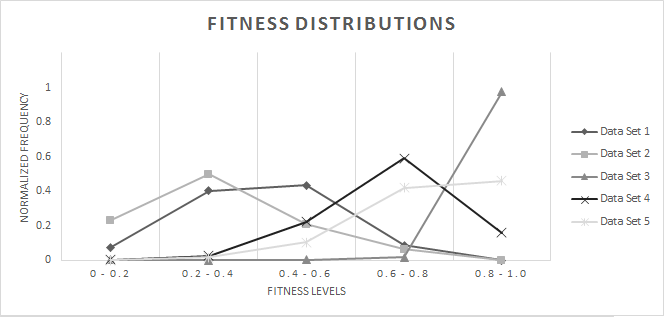
\includegraphics[width=\linewidth]{fitness-dist}
\end{figure}

The hamming distance in a level (HDIL) is indicative of the width of the landscape for the different fitness levels. In other words, how clustered the solutions within the specific fitness level are. Since Hamming Distance measures the number of bits that differ between two bit strings, the maximum possible hamming distance between two bit strings is the length of the bit string. The length of the bit string for the discrete landscape is the dimensionality,  $I$, of the problem.
Table \ref{dim} shows the HDIL difference with respect to the dimensionality of the problem.

 \begin{table}[H]
\centering
\caption{HDIL difference with respect to the dimensions of the problem}
\label{dim}
\begin{tabular}{lll}
\textbf{Data Set 1 ($I = 70$)} & HDIL & Dimensional Difference \\ \hline
\multicolumn{1}{|l|}{$ f(x) < $ 0.2} & \multicolumn{1}{l|}{37.2943} & \multicolumn{1}{l|}{0.5328} \\ \hline
\multicolumn{1}{|l|}{0.2 $ < f(x) \leq $ 0.4} & \multicolumn{1}{l|}{35.8924} & \multicolumn{1}{l|}{0.5127} \\ \hline
\multicolumn{1}{|l|}{0.4 $ < f(x) \leq $ 0.6} & \multicolumn{1}{l|}{35.8436} & \multicolumn{1}{l|}{0.5121} \\ \hline
\multicolumn{1}{|l|}{0.6 $ < f(x) \leq $ 0.8} & \multicolumn{1}{l|}{37.0920} & \multicolumn{1}{l|}{0.5299} \\ \hline
\multicolumn{1}{|l|}{0.8 $ < f(x) \leq $ 1.0} & \multicolumn{1}{l|}{0.0000} & \multicolumn{1}{l|}{0.0000} \\ \hline
\textbf{Data Set 2 ($I = 5$)} & \\ \hline
\multicolumn{1}{|l|}{$ f(x) < $ 0.2} & \multicolumn{1}{l|}{3.8712} & \multicolumn{1}{l|}{0.7742} \\ \hline
\multicolumn{1}{|l|}{0.2 $ < f(x) \leq $ 0.4} & \multicolumn{1}{l|}{3.0076} & \multicolumn{1}{l|}{0.6015} \\ \hline
\multicolumn{1}{|l|}{0.4 $ < f(x) \leq $ 0.6} & \multicolumn{1}{l|}{3.6805} & \multicolumn{1}{l|}{0.7361} \\ \hline
\multicolumn{1}{|l|}{0.6 $ < f(x) \leq $ 0.8} & \multicolumn{1}{l|}{5.0000} & \multicolumn{1}{l|}{1.0000} \\ \hline
\multicolumn{1}{|l|}{0.8 $ < f(x) \leq $ 1.0} & \multicolumn{1}{l|}{0.0000} & \multicolumn{1}{l|}{0.0000} \\ \hline
\textbf{Data Set 3 ($I = 10$)} &   \\ \hline
\multicolumn{1}{|l|}{$ f(x) < $ 0.2} & \multicolumn{1}{l|}{10.0000} & \multicolumn{1}{l|}{1.0000} \\ \hline
\multicolumn{1}{|l|}{0.2 $ < f(x) \leq $ 0.4} & \multicolumn{1}{l|}{0.0000} & \multicolumn{1}{l|}{0.0000} \\ \hline
\multicolumn{1}{|l|}{0.4 $ < f(x) \leq $ 0.6} & \multicolumn{1}{l|}{9.0278} & \multicolumn{1}{l|}{0.9028} \\ \hline
\multicolumn{1}{|l|}{0.6 $ < f(x) \leq $ 0.8} & \multicolumn{1}{l|}{7.6767} & \multicolumn{1}{l|}{0.7677} \\ \hline
\multicolumn{1}{|l|}{0.8 $ < f(x) \leq $ 1.0} & \multicolumn{1}{l|}{5.5266} & \multicolumn{1}{l|}{0.5527} \\ \hline
\textbf{Data Set 4 ($I = 39$)} &   \\ \hline
\multicolumn{1}{|l|}{$ f(x) < $ 0.2} & \multicolumn{1}{l|}{26.9497} & \multicolumn{1}{l|}{0.6910} \\ \hline
\multicolumn{1}{|l|}{0.2 $ < f(x) \leq $ 0.4} & \multicolumn{1}{l|}{22.5481} & \multicolumn{1}{l|}{0.5782} \\ \hline
\multicolumn{1}{|l|}{0.4 $ < f(x) \leq $ 0.6} & \multicolumn{1}{l|}{20.5674} & \multicolumn{1}{l|}{0.5274} \\ \hline
\multicolumn{1}{|l|}{0.6 $ < f(x) \leq $ 0.8} & \multicolumn{1}{l|}{20.0692} & \multicolumn{1}{l|}{0.5146} \\ \hline
\multicolumn{1}{|l|}{0.8 $ < f(x) \leq $ 1.0} & \multicolumn{1}{l|}{21.2160} & \multicolumn{1}{l|}{0.5440} \\ \hline
\textbf{Data Set 5 ($I = 16$)} &  \\ \hline
\multicolumn{1}{|l|}{$ f(x) < $ 0.2} & \multicolumn{1}{l|}{14.4400} & \multicolumn{1}{l|}{0.9025} \\ \hline
\multicolumn{1}{|l|}{0.2 $ < f(x) \leq $ 0.4} & \multicolumn{1}{l|}{11.5693} & \multicolumn{1}{l|}{0.7231} \\ \hline
\multicolumn{1}{|l|}{0.4 $ < f(x) \leq $ 0.6} & \multicolumn{1}{l|}{10.1475} & \multicolumn{1}{l|}{0.6342} \\ \hline
\multicolumn{1}{|l|}{0.6 $ < f(x) \leq $ 0.8} & \multicolumn{1}{l|}{9.1494} & \multicolumn{1}{l|}{0.5718} \\ \hline
\multicolumn{1}{|l|}{0.8 $ < f(x) \leq $ 1.0} & \multicolumn{1}{l|}{9.4104} & \multicolumn{1}{l|}{0.5882} \\ \hline
\end{tabular}
\end{table}

 In order to compare the HDIL values for the different data sets the HDIL values are normalized linearly to the same 0 to 1 scale as with the fitness distribution frequencies, called Dimensional Difference, in table \ref{dim}. Dimensionality Difference is calculated as $ D(L) = HDIL(L)/I$, where $L$ is the fitness level. The HDIL measure is essentially the average Hamming Distance between solutions in a level. The Dimensional Difference thus shows by how much solutions in a level differed with respect to the dimensionality of the problem. As can be observed, a commonality can be seen between all the tested levels and data sets. The minimum observed Dimensionality Difference for all levels is $0.5121$. It can thus be said that for such high HDIL values, the specific bit strings (solutions) in all levels are not close together or clustered in a group. This does not however mean that they do not form part of a larger cluster that spans multiple levels.


% An example of a floating figure using the graphicx package.
% Note that \label must occur AFTER (or within) \caption.
% For figures, \caption should occur after the \includegraphics.
% Note that IEEEtran v1.7 and later has special internal code that
% is designed to preserve the operation of \label within \caption
% even when the captionsoff option is in effect. However, because
% of issues like this, it may be the safest practice to put all your
% \label just after \caption rather than within \caption{}.
%
% Reminder: the "draftcls" or "draftclsnofoot", not "draft", class
% option should be used if it is desired that the figures are to be
% displayed while in draft mode.
%
%\begin{figure}[!t]
%\centering
%\includegraphics[width=2.5in]{myfigure}
% where an .eps filename suffix will be assumed under latex, 
% and a .pdf suffix will be assumed for pdflatex; or what has been declared
% via \DeclareGraphicsExtensions.
%\caption{Simulation results for the network.}
%\label{fig_sim}
%\end{figure}

% Note that the IEEE typically puts floats only at the top, even when this
% results in a large percentage of a column being occupied by floats.


% An example of a double column floating figure using two subfigures.
% (The subfig.sty package must be loaded for this to work.)
% The subfigure \label commands are set within each subfloat command,
% and the \label for the overall figure must come after \caption.
% \hfil is used as a separator to get equal spacing.
% Watch out that the combined width of all the subfigures on a 
% line do not exceed the text width or a line break will occur.
%
%\begin{figure*}[!t]
%\centering
%\subfloat[Case I]{\includegraphics[width=2.5in]{box}%
%\label{fig_first_case}}
%\hfil
%\subfloat[Case II]{\includegraphics[width=2.5in]{box}%
%\label{fig_second_case}}
%\caption{Simulation results for the network.}
%\label{fig_sim}
%\end{figure*}
%
% Note that often IEEE papers with subfigures do not employ subfigure
% captions (using the optional argument to \subfloat[]), but instead will
% reference/describe all of them (a), (b), etc., within the main caption.
% Be aware that for subfig.sty to generate the (a), (b), etc., subfigure
% labels, the optional argument to \subfloat must be present. If a
% subcaption is not desired, just leave its contents blank,
% e.g., \subfloat[].


% An example of a floating table. Note that, for IEEE style tables, the
% \caption command should come BEFORE the table and, given that table
% captions serve much like titles, are usually capitalized except for words
% such as a, an, and, as, at, but, by, for, in, nor, of, on, or, the, to
% and up, which are usually not capitalized unless they are the first or
% last word of the caption. Table text will default to \footnotesize as
% the IEEE normally uses this smaller font for tables.
% The \label must come after \caption as always.
%
%\begin{table}[!t]
%% increase table row spacing, adjust to taste
%\renewcommand{\arraystretch}{1.3}
% if using array.sty, it might be a good idea to tweak the value of
% \extrarowheight as needed to properly center the text within the cells
%\caption{An Example of a Table}
%\label{table_example}
%\centering
%% Some packages, such as MDW tools, offer better commands for making tables
%% than the plain LaTeX2e tabular which is used here.
%\begin{tabular}{|c||c|}
%\hline
%One & Two\\
%\hline
%Three & Four\\
%\hline
%\end{tabular}
%\end{table}


% Note that the IEEE does not put floats in the very first column
% - or typically anywhere on the first page for that matter. Also,
% in-text middle ("here") positioning is typically not used, but it
% is allowed and encouraged for Computer Society conferences (but
% not Computer Society journals). Most IEEE journals/conferences use
% top floats exclusively. 
% Note that, LaTeX2e, unlike IEEE journals/conferences, places
% footnotes above bottom floats. This can be corrected via the
% \fnbelowfloat command of the stfloats package.

\section{Conclusion}

Taking the fitness distributions into consideration, it is evident that there is little commonality between fitness distributions for a given classifier and a variety of problems using a specific subset of features. This could likely be due to the simplicity of the classifier that is used. Investigating the fitness distributions for a set of classifiers on a set of problems could perhaps provide for a better profiling of the feature selection problem. 

Finally, for the different fitness levels it was found that solutions within all levels are highly scattered throughout the level, with an average of at least $51\%$ difference between bit strings within any level. This finding can be applied to further the development of new techniques for feature selection, or the improvement of existing techniques. Heuristic based techniques could possibly greatly benefit from prior knowledge of such structural elements in the feature selection search space. 

Future work will include investigating the link between fitness landscape features and the performance of algorithms for the feature selection problem.


% if have a single appendix:
%\appendix[Proof of the Zonklar Equations]
% or
%\appendix  % for no appendix heading
% do not use \section anymore after \appendix, only \section*
% is possibly needed

% use appendices with more than one appendix
% then use \section to start each appendix
% you must declare a \section before using any
% \subsection or using \label (\appendices by itself
% starts a section numbered zero.)
%

%\appendices
%\section{Proof of the First Zonklar Equation}
%Appendix one text goes here.

%The authors would like to thank...

% Can use something like this to put references on a page
% by themselves when using endfloat and the captionsoff option.
\ifCLASSOPTIONcaptionsoff
  \newpage
\fi


% trigger a \newpage just before the given reference
% number - used to balance the columns on the last page
% adjust value as needed - may need to be readjusted if
% the document is modified later
%\IEEEtriggeratref{8}
% The "triggered" command can be changed if desired:
%\IEEEtriggercmd{\enlargethispage{-5in}}

% references section

% can use a bibliography generated by BibTeX as a .bbl file
% BibTeX documentation can be easily obtained at:
% http://mirror.ctan.org/biblio/bibtex/contrib/doc/
% The IEEEtran BibTeX style support page is at:
% http://www.michaelshell.org/tex/ieeetran/bibtex/
%\bibliographystyle{IEEEtran}
% argument is your BibTeX string definitions and bibliography database(s)
%\bibliography{IEEEabrv,../bib/paper}
%

\bibliographystyle{IEEEtran} 
\bibliography{references}
% that's all folks
\end{document}


